% 目次の挿入
\tableofcontents
\newpage

% ヘッダーカスタマイズ
\pagestyle{fancy}
\fancyhf{}
\fancyhead[L]{DLITE3:Technology that supports people's lives without boundaries}
\renewcommand{\headrulewidth}{0pt}
\makeatletter
\let\ps@plain\ps@fancy
\makeatother
% ヘッダーの下に空白を追加
\setlength{\headsep}{20pt}

\chapter{はじめに}
\section{背景}
適当な例で本文を書いていくので、chapterやsectionを含め本文を自由に改変してください。\\
朝、目覚まし時計が鳴り目が覚めた後、目覚まし時計まで手が届かず止めるのが困難である。
\begin{figure}[h!]
  \centering
  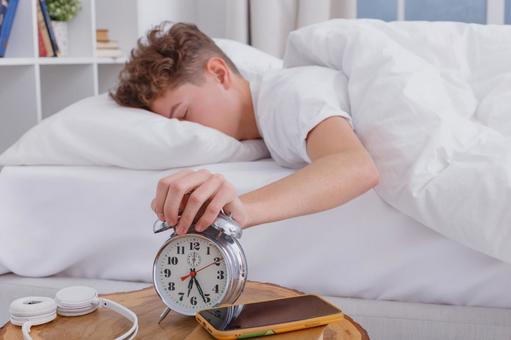
\includegraphics[width=0.8\textwidth]{pages/report/images/alarm-stopping.jpeg}
  \caption{目覚ましの停止が困難な図}
  \label{fig:sample}
\end{figure}
\writer{未来太郎}

\section{先行研究}
コダマ2024\cite{目覚まし時計を改造}によると、目覚まし時計を本体についているボタンとは別に停止する改造はすでに行われている。
しかし、その改造は目覚まし時計の本体に直接改造を加えるものであり、目覚まし時計の本体に直接改造を加えることは、目覚まし時計の保証が無効になる可能性がある。
また、ボタンの延長はケーブルで行われており、夜中布団から出るときなどに転倒の原因となる可能性があり、安全性に問題がある。
\writer{未来太郎}

\section{研究動機}
目覚まし時計がなることにより目が覚めた後、目覚まし時計を止めないことに快適な二度寝を楽しむことが出来ない。
そのため、目覚まし時計を止めることが容易になるような方法を考えることが必要であると考えた。
実際に、起床時にアラームで起きた際にどのような問題が生じるのかについてフィールドワークを行ったところ、布団から出て目覚まし時計を停止させることで目が覚めてしまい、快適な二度寝が出来ないことが判明した。
\writer{未来太郎}

\section{目的及び重要性}
布団から一歩も出ずに用意に目覚まし時計を止めることが出来るような方法を考案することで、快適な二度を実現する。
また、快適な二度寝により幸福度が増し、生活の質が向上することが期待されるとともに、人生を豊かにすることが出来ると考える。
\writer{未来太郎}

\chapter{関連研究}
\section{必要なスキル}
遠隔操作により、ワイヤレスで目覚まし時計を操作することが出来るような方法を考案することが必要である。
また、そのためには以下の技術の習得が必要であると考える。
\begin{itemize}
    \item ワイヤレス通信技術
    \item マイコン制御技術
    \item 電子回路設計技術
    \item スマホアプリ開発技術
\end{itemize}
\writer{未来太郎}

\section{解決方法・手法}
目覚まし時計を止めるための方法として、ワイヤレスで目覚まし時計を操作する方法を考案する。
目覚まし時計が作動しし目が覚めた後、スマホを操作することで目覚まし時計の停止ボタンが遠隔で押されるようにする。
目覚まし時計本体の改造を行わなくても良いように、外付けが可能なデバイスを作成する。
\writer{未来太郎}

\chapter{本プロジェクト学習の目標}
\section{最終的な目標}
本プロジェクト学習では、目覚まし時計をスマホで操作し遠隔で停止させるアプリ、デバイスを開発することで、快適な二度寝を実現することを目標とする。
またそれにより、生活の質が向上し、幸福度を増加させることを最終的な目標とする。
\writer{未来太郎}

\chapter{目的を達成するための手法・手段}
\section{考案したアイデア}
考案したアイデアについて述べる。
\writer{未来太郎}

\section{新しい解決方法・手法}
解決方法の新規性について述べたりする。
\writer{未来太郎}

\section{用いる技術}
上記を実現するために用いる技術について述べる。
\writer{未来太郎}

\chapter{結果}
\section{手法な結果}
どんな結果が得られたのかを事実に基づいて述べる。
\writer{未来太郎}

\chapter{考察}
\section{得られた成果}
本プロジェクト学習を通じてどのような成果を得られ、どのような効果が発生したのかについて考察する。
\writer{未来太郎}

\section{妥当性}
得られた結果は妥当かどうかについて述べる。
\writer{未来太郎}

\section{課題点}
用いた手法、技術では得られなかったことについて述べる。
\writer{未来太郎}

\section{本学との関連性}
本学のカリキュラムや講義科目との関係や関連性について述べる。
\writer{未来太郎}

\section{拡張性}
本プロジェクト学習を拡張することでどのような新たなテーマが考えられるかについて述べる。
\writer{未来太郎}

\section{今後の展望}
今後の展望について述べる。
\writer{未来太郎}

\newpage\clearpage
\vspace*{-20pt}
\addcontentsline{toc}{chapter}{参考文献}  % 目次に「参考文献」を追加
\printbibliography[segment=\therefsegment,heading=subbibliography]
